\documentclass{article}

% Language setting
\usepackage[english]{babel}

% Page size and margins
\usepackage[letterpaper,top=2cm,bottom=2cm,left=3cm,right=3cm,marginparwidth=1.75cm]{geometry}

% Packages
\usepackage{amsmath, amssymb, amsthm}
\usepackage{color}
\usepackage{xcolor}
\usepackage{indentfirst}
\usepackage{graphicx}
\usepackage{makecell}
\usepackage{listings}
\usepackage{array}
\usepackage{mathpazo}
\usepackage{csquotes}

\usepackage[
    style=ext-numeric,
    sorting=none,
    backend=biber,
    date=long,
    dateabbrev=false
]{biblatex}

% Bibliography file
\addbibresource{references.bib}


% Title font
\newcommand{\titlefont}{\fontfamily{ppl}\selectfont}
\usepackage{titlesec}
\usepackage{colortbl}
\usepackage{makecell}
\usepackage{multirow}
\usepackage{tabularx}
\usepackage[most]{tcolorbox}
\usepackage{soul}
\usepackage{fancyhdr}
\usepackage{tikz}
\usepackage{booktabs}
\usepackage{mdframed}
\usepackage{enumitem}
\usepackage[colorlinks=true, allcolors=blue]{hyperref}
\usetikzlibrary{decorations,positioning,shapes.geometric,arrows.meta,fit,backgrounds}
\usetikzlibrary{petri}

% Custom colors
\definecolor{codegreen}{rgb}{0,0.6,0}
\definecolor{codegray}{rgb}{0.5,0.5,0.5}
\definecolor{codepurple}{rgb}{0.58,0,0.82}
\definecolor{backcolour}{rgb}{0.95,0.95,0.92}

\pagestyle{fancy}

% Clear headers and footers
\fancyhead{}
\fancyfoot{}
\lstdefinestyle{mystyle}{
    backgroundcolor=\color{backcolour},
    commentstyle=\color{codegreen},
    keywordstyle=\color{magenta},
    numberstyle=\tiny\color{codegray},
    stringstyle=\color{codepurple},
    basicstyle=\ttfamily\footnotesize,
    breakatwhitespace=false,
    breaklines=true,
    captionpos=b,
    keepspaces=true,
    numbers=left,
    numbersep=5pt,
    showspaces=false,
    showstringspaces=false,
    showtabs=false,
    tabsize=2
}

\lstset{style=mystyle}

\lhead{Instructor: Prof. Sharon Myers}
\rhead{Counterattacking Botnets.}
\lfoot{English 202C, Spring 2025, Instruction Set}
\cfoot{\thepage}
\rfoot{UC Choudhary (ufc5009)}

\begin{document}
\begin{titlepage}
  \vspace*{160pt}
  \begin{center}
    {\titlefont \Huge Counterattacking Botnets.}\\[1cm]
    {\LARGE Name: UC Choudhary\\[1cm]}
    {\LARGE PSU email: ufc5009@psu.edu\\[1cm]}
    {\LARGE PSU ID: 971854622\\[1cm]}
  \end{center}
  \thispagestyle{fancy}
  \vspace*{\fill}
\end{titlepage}

\tableofcontents
\newpage

\begin{tcolorbox}[
  colback=backcolour,            % background color
  colframe=red!75!black,    % border color
  title={Disclaimer},
  fonttitle=\bfseries\large\centering,
  arc=4mm,                  % rounded corners
  boxrule=1pt,              % border thickness
  left=10pt, right=10pt,    % inner horizontal padding
  top=10pt, bottom=10pt,    % inner vertical padding
  enhanced
]
Malicious use of a botnet is a cybercrime and a serious criminal offense!
Everything in this article is for educational purposes only.
\end{tcolorbox}
\section{Introduction}
\noindent A botnet is the weapon of choice for organized hacking groups like Anonymous, LulzSec etc. because it allows the attackers to wield the most powerful attack mechanism invented. Before we get into how to fight a botnet, we need to learn a little about botnets. A botnet can launch a swarm of attacks simultaneously.  This allows the attackers to gauge and exploit weaknesses depending on data collected by the attack. The size of a botnet in reality has no limit, it depends on the resources that the attacker or group of attackers have. Organized hacking groups can leverage this and orchestrate multiple botnet attacks at the same time.
In simple terms, a botnet is a collection of compromise (puppet) computers under the control of a central C2(Command and Control) server (the puppet master). Figure 1 is a very accurate representation of a botnet.
\begin{tcolorbox}[
  colback=backcolour,            % background color
  colframe=blue!75!black,    % border color
  title={Botnet},
  fonttitle=\bfseries\large\centering,
  arc=4mm,                  % rounded corners
  boxrule=1pt,              % border thickness
  left=10pt, right=10pt,    % inner horizontal padding
  top=10pt, bottom=10pt,    % inner vertical padding
  enhanced
]
% \begin{figure}[h!]
    \includegraphics[width=\linewidth]{bnstruc.png}
    \begin{center}
    The structure of a botnet.$^{\text{\href{https://www.a10networks.com/wp-content/uploads/how-a-bot-herder-attacks.png}{[7]}}}$
    \end{center}
% \end{figure}
\end{tcolorbox}

\subsection{White-Hat Worms and PN2 Modeling}
Inspired by the extended Hajime worm model, our white-hat worm incorporates:
\begin{itemize}
    \item \textbf{Lifespan:} A predetermined operational period after which the worm self-destructs, preventing persistent presence.
    \item \textbf{Secondary Infectivity:} The ability to infect devices already compromised by malware, thereby displacing malicious agents.
    \item \textbf{C2 Disruption:} Mechanisms to intercept and disrupt the botnet's command-and-control communications.
\end{itemize}
These features are modeled using agent-oriented Petri nets (PN2), which allow us to simulate and evaluate interactions between malicious malware (e.g., Mirai) and our defensive worm.

\begin{tcolorbox}[
    colback=blue!5!white, 
    colframe=black!75!black, 
    title={Deception Tactic Workflow}, 
    fonttitle=\bfseries\large\centering,
    arc=4mm,                  
    boxrule=1pt,              
    left=10pt, right=10pt,    
    top=10pt, bottom=10pt,    
    enhanced
]
\noindent To enhance threat intelligence through controlled deception, we can use a tactic leveraging the Cowrie honeypot's interactive environment.

\subsection*{Workflow: Deception-Based Intelligence Gathering}

\noindent \textbf{Step 1: Initial Connection} \\
An attacker connects to the Cowrie honeypot, unaware of its deceptive nature:
\begin{lstlisting}[language=bash, caption={Attacker Session Initiation}, label={lst:step1}]
$ ssh attacker@honeypot-ip
Welcome to Cowrie SSH Honeypot!
$ whoami
Response: user@fake-server
\end{lstlisting}

\noindent \textbf{Step 2: Deceptive Prompt Activation} \\
The honeypot presents a fabricated privilege escalation prompt:
\begin{lstlisting}
Enter your username to escalate privileges:
\end{lstlisting}
The attacker inputs their real username, believing this to be a genuine system interaction:
\begin{lstlisting}[language=bash, caption={Attacker Credential Disclosure}, label={lst:step2}]
realuser
\end{lstlisting}

\noindent \textbf{Step 3: Data Correlation} \\
Cowrie automatically logs the attacker's input alongside metadata:
\begin{itemize}
    \item Username: \texttt{realuser} (from Listing \ref{lst:step2})
    \item Source IP: \texttt{192.168.X.X} (from connection metadata)
    \item Timestamp: \texttt{2025-03-25T14:30:00Z}
\end{itemize}

\subsection*{Operational Constraints}
\begin{mdframed}[backgroundcolor=yellow!10, linewidth=1pt]
\noindent \textbf{Important Considerations:} \\
While Cowrie creates an illusion of vulnerability, it \emph{cannot} execute commands on attackers' systems [[8]]. This workflow strictly serves defensive intelligence purposes, aligning with recommendations from [[3]] and [[6]] to avoid active countermeasures.
\end{mdframed}
\end{tcolorbox}
\section{Design of the Counterattack Worm}
\noindent
This section details the architecture of an advanced counterattack worm that not only neutralizes malware infections but also disrupts the botnet’s C2 infrastructure.

\subsection{Key Features}
The counterattack worm is designed with the following characteristics:
\begin{itemize}
    \item \textbf{Lifespan and Self-Destruction:} The worm operates only for a short, pre-defined time before self-destructing to avoid collateral damage.
    \item \textbf{Secondary Infectivity:} It can infect devices that are already compromised by malicious botnets, thereby removing the harmful agent.
    \item \textbf{C2 Disruption:} It includes routines to identify and disrupt the command-and-control channels of the malicious botnet. This is achieved by intercepting network communications, injecting false commands, or jamming signals between the botnet and its C2 server.
\end{itemize}

\subsection{C2 Disruption Mechanism}
The worm's C2 disruption module operates as follows:
\begin{enumerate}
    \item \textbf{Network Scanning:} The worm scans for known C2 server signatures based on historical data and threat intelligence feeds.
    \item \textbf{Interception and Spoofing:} Once a C2 server is identified, the worm intercepts outgoing communication from the infected device and injects false commands. This can lead the malicious bot to cease operations or redirect its commands.
    \item \textbf{Self-Limiting Operation:} After executing its countermeasures, the worm logs the disruption event and terminates its process to prevent extended interference.
\end{enumerate}

\subsection{Implementation in a Simulated Environment}
The deployment environment consists of Docker-based Cowrie honeypots and simulated IoT devices. The worm operates within a controlled network where its actions can be monitored and evaluated using a PN2 model.

\section{Simulation Environment and PN2 Modeling}
\noindent
To evaluate the effectiveness of both the deception tactic and the counterattack worm, we utilize a simulation environment modeled with PN2. The extended PN2 model includes states for:
\begin{itemize}
    \item \textbf{Mirai Infection:} Representing the propagation of the malicious botnet.
    \item \textbf{White-Hat Worm Infection:} Incorporating lifespan, secondary infectivity, and C2 disruption.
    \item \textbf{Device State Transitions:} Showing transitions from an infected state to a neutralized state following worm intervention.
\end{itemize}

\subsection{Example PN2 Diagram with C2 Disruption}
\begin{figure}[h]
\centering
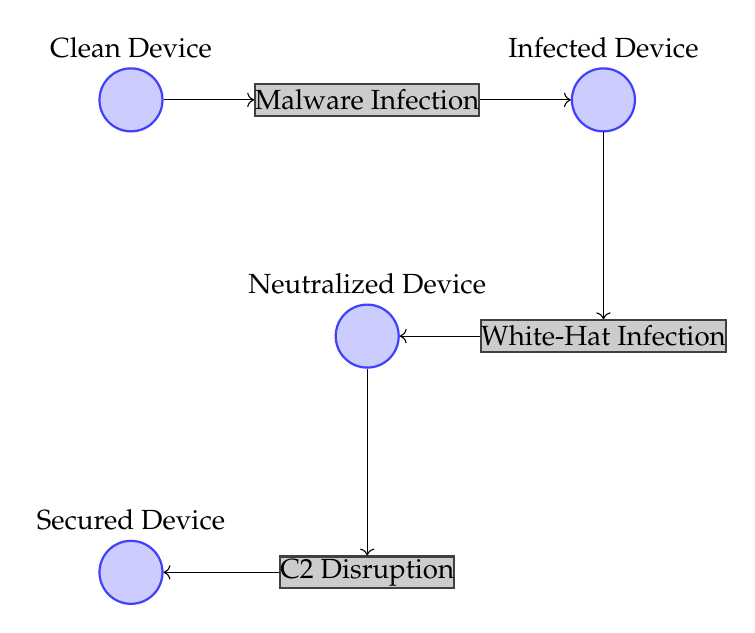
\begin{tikzpicture}[node distance=3cm, on grid, auto,
    every place/.style={draw=blue!75, fill=blue!20, thick, minimum size=8mm},
    every transition/.style={draw=black!75, fill=black!20, thick},
    bend angle=45]
    % Places
    \node[place] (clean) [label=above:Clean Device] {};
    \node[transition] (mal_infect) [right=of clean] {Malware Infection};
    \node[place] (infected) [right=of mal_infect, label=above:Infected Device] {};
    \node[transition] (white_infect) [below=of infected] {White-Hat Infection};
    \node[place] (neutralized) [left=of white_infect, label=above:Neutralized Device] {};
    \node[transition] (c2_disrupt) [below=of neutralized] {C2 Disruption};
    \node[place] (secured) [left=of c2_disrupt, label=above:Secured Device] {};
    
    % Arrows
    \draw[->] (clean) -- (mal_infect);
    \draw[->] (mal_infect) -- (infected);
    \draw[->] (infected) -- (white_infect);
    \draw[->] (white_infect) -- (neutralized);
    \draw[->] (neutralized) -- (c2_disrupt);
    \draw[->] (c2_disrupt) -- (secured);
\end{tikzpicture}
\caption{Simplified PN2 model including C2 disruption.}
\label{fig:pn2_c2}
\end{figure}

\subsection{Simulation Evaluation}
The simulation measures:
\begin{itemize}
    \item \textbf{Infection Rates:} The percentage of devices infected by Mirai versus those neutralized by the white-hat worm.
    \item \textbf{Disruption Effectiveness:} How effectively the C2 channels are interrupted.
    \item \textbf{Worm Lifespan and Secondary Infectivity:} The trade-offs between rapid self-destruction and prolonged protective coverage.
\end{itemize}
The results—derived from thousands of simulation trials—indicate that high secondary infectivity combined with effective C2 disruption leads to a rapid decline in malicious botnet activity while limiting collateral damage.

\section{Deployment and Operation of the C2 Disruption Mechanism}
\noindent
This section provides a full instruction set detailing multiple steps to deploy and use the C2 disruption mechanism.

\subsection{Step 1: Environment Setup}
\begin{enumerate}
    \item Install Python 3.x and the required packages. Ensure that Scapy is installed:
    \begin{lstlisting}[language=bash]
pip install scapy
    \end{lstlisting}
    \item Configure your network environment in a controlled lab setting. Use Docker-based Cowrie honeypots and simulated IoT devices to ensure no unintended interference with production systems.
\end{enumerate}

\subsection{Step 2: Configure the Network Interface}
\begin{enumerate}
    \item Identify the network interface to monitor (e.g., \texttt{eth0}).
    \item In the provided Python script (see Section~\ref{sec:python_code} below), set the \texttt{interface} variable to your desired network interface.
\end{enumerate}

\subsection{Step 3: Deploy the Python Script}
\begin{enumerate}
    \item Save the following Python code (see Section~\ref{sec:python_code}) as \texttt{c2\_disruption.py}.
    \item Ensure the script has execute permissions:
    \begin{lstlisting}[language=bash]
chmod +x c2_disruption.py
    \end{lstlisting}
\end{enumerate}

\subsection{Step 4: Execute the C2 Disruption Mechanism}
\begin{enumerate}
    \item Run the script in your controlled environment:
    \begin{lstlisting}[language=bash]
python c2_disruption.py
    \end{lstlisting}
    \item The script will begin monitoring the network traffic on the specified interface. It will inspect each packet and check for known malicious C2 signatures.
\end{enumerate}

\subsection{Step 5: Monitor and Log the Operations}
\begin{enumerate}
    \item The script logs all events with timestamps, including normal packet summaries, detected malicious C2 traffic, and disruption actions.
    \item Review the log output in the console or redirect output to a file for further forensic analysis.
\end{enumerate}

\subsection{Step 6: Evaluate Disruption Effectiveness}
\begin{enumerate}
    \item After running the script for a sufficient period, analyze the logs to determine:
    \begin{itemize}
        \item The number of intercepted C2 communications.
        \item The frequency of false command injections.
        \item Any anomalies in network traffic that indicate successful disruption.
    \end{itemize}
    \item Compare these findings with simulation data from the PN2 model to validate the operational effectiveness.
\end{enumerate}

\subsection{Step 7: Shutdown and Cleanup}
\begin{enumerate}
    \item Once testing is complete, gracefully terminate the script (e.g., using CTRL+C). The script will log a shutdown message.
    \item Review all logs, document the findings, and remove any temporary files or configuration changes.
\end{enumerate}

\subsection{Section: Python Code for C2 Disruption Mechanism}
\label{sec:python_code}
Below is the complete Python code implementing the C2 disruption mechanism:
\begin{lstlisting}[language=Python, caption={Python Code for C2 Disruption Mechanism}]
import time
from scapy import sniff, send, IP, Raw

def load_malicious_signatures():
    """
    Load a list of known malicious C2 signatures.
    In practice, these should be derived from threat intelligence.
    """
    return ["malicious_command", "C2_COMMAND", "EVIL_PAYLOAD"]

def log_event(event_message):
    """
    Logs an event with a timestamp.
    """
    timestamp = time.strftime("%Y-%m-%d %H:%M:%S", time.localtime())
    print(f"{timestamp}: {event_message}")

def report_event(event_message):
    """
    Reports an event to a centralized white-hat C2 server.
    This is a placeholder function – implement secure transmission as needed.
    """
    log_event(f"Reporting event: {event_message}")

def generate_false_command():
    """
    Generates a false command intended to disable the malicious bot.
    """
    return "DISABLE_MALWARE"

def is_malicious_C2(packet):
    """
    Checks whether a packet contains a malicious C2 signature.
    """
    signatures = load_malicious_signatures()
    if packet.haslayer(Raw):
        try:
            payload = packet[Raw].load.decode('utf-8', errors='ignore')
        except Exception as e:
            log_event(f"Error decoding packet payload: {e}")
            return False
        for signature in signatures:
            if signature in payload:
                return True
    return False

def drop_packet(packet):
    """
    Simulates dropping a packet.
    In practice, you might use firewall rules or other network-level controls.
    """
    log_event(f"Packet dropped: {packet.summary()}")

def inject_packet(ip_address, false_command):
    """
    Creates and sends a packet with a false command to the specified IP address.
    """
    new_packet = IP(dst=ip_address) / Raw(load=false_command)
    send(new_packet, verbose=False)
    log_event(f"Injected false command to IP {ip_address}")

def disrupt_C2(packet):
    """
    Disrupts the malicious C2 communication by dropping the packet
    and injecting a false command.
    """
    if IP in packet:
        target_ip = packet[IP].dst
        log_event(f"C2 disruption initiated on IP {target_ip}")
        drop_packet(packet)
        false_command = generate_false_command()
        inject_packet(target_ip, false_command)
        report_event(f"Disrupted C2 communication on {target_ip}. False command injected.")

def packet_callback(packet):
    """
    Callback function for each captured packet.
    Checks if the packet is part of a malicious C2 communication.
    """
    if is_malicious_C2(packet):
        disrupt_C2(packet)
    else:
        log_event("Normal packet: " + packet.summary())

def monitor_network(interface):
    """
    Continuously monitors network traffic on the specified interface.
    """
    log_event(f"Starting network monitoring on interface {interface}")
    sniff(iface=interface, prn=packet_callback, store=0)

if __name__ == "__main__":
    # Set the interface to monitor (change as needed)
    interface = "eth0"
    try:
        monitor_network(interface)
    except KeyboardInterrupt:
        log_event("Network monitoring stopped by user")
\end{lstlisting}
\clearpage
\begin{tcolorbox}[
  colback=backcolour,            % background color
  colframe=red!75!black,    % border color
  title={Ethical and Legal Considerations},
  fonttitle=\bfseries\large\centering,
  arc=4mm,                  % rounded corners
  boxrule=1pt,              % border thickness
  left=10pt, right=10pt,    % inner horizontal padding
  top=10pt, bottom=10pt,    % inner vertical padding
  enhanced
]
\noindent
The use of white-hat worms, even in theoretical and simulated environments, raises serious ethical and legal issues. It is crucial to emphasize that:
\begin{itemize}
    \item All experiments must be conducted in controlled, isolated environments with explicit authorization.
    \item The intent is solely defensive—to improve threat intelligence and bolster cybersecurity measures.
    \item Unauthorized deployment of such techniques in public networks is illegal and unethical.
\end{itemize}
\end{tcolorbox}

\section{Conclusion and Future Work}
\noindent
This instruction set presents an advanced approach to counterattacking botnets by combining deception tactics with a defensive white-hat worm capable of C2 disruption. Key innovations include:
\begin{itemize}
    \item A detailed deception workflow using a simulated Cowrie honeypot to capture attacker data.
    \item The design of a counterattack worm that not only displaces malicious code but also disrupts botnet C2 channels.
    \item A robust simulation framework using PN2 models to quantitatively assess the efficacy of the defensive measures.
    \item A comprehensive, step-by-step instruction set for deploying and operating the C2 disruption mechanism.
\end{itemize}
Future work will focus on refining the C2 disruption algorithms and integrating machine learning to dynamically adjust worm parameters based on real-time threat intelligence.

\section{Glossary of Technical Terms}
\begin{itemize}
    \item \textbf{Botnet:} A network of compromised devices under centralized control.
    \item \textbf{Honeypot:} A decoy system designed to lure attackers and capture their activity.
    \item \textbf{White-Hat Worm:} A benevolent worm engineered to counteract malicious malware.
    \item \textbf{PN2 (Petri Net in a Petri Net):} A modeling approach for multi-agent systems that allows nested state transitions.
    \item \textbf{C2 (Command and Control):} The infrastructure through which a botnet receives instructions from its controller.
\end{itemize}


\nocite{*}
\printbibliography[heading=bibintoc,title={References}]
\end{document}
